\chapter{Projekt i implementacja}

\section{Wykorzystane technologie}
\subsection{Python 3.8.1}
Do implementacji algorytmu został użyty Python. Jest to najpopularniejszy język programowania w domenie uczenia maszynowego. Wymagana jest wersja 3.8+ ze względu na użycie w implementacji metod dostępnych od tej wersji.  
\subsection{PonyGE2}
PonyGE2 \cite{Fenton_2017} jest implementacja ewolucji genetycznej w jezyku Python. Pozwala na latwa konfiguracje parametrow ewolucji genetycznej oraz latwa mozliwosc dodania wlasnych problemow oraz sposobow ewaluacji wynikow.

\begin{figure}[h]
	\centering{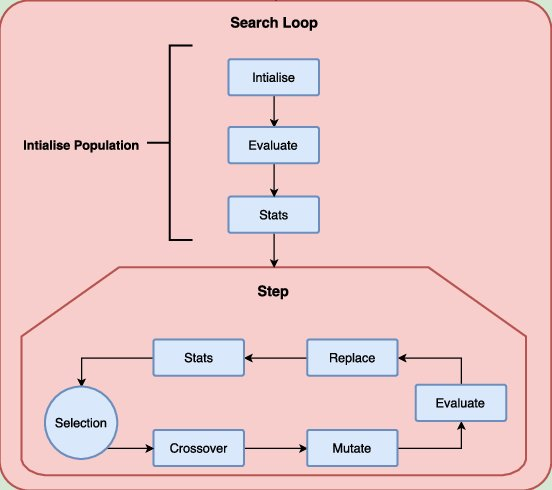
\includegraphics{PonyGE2-search-loop.jpg}}
	\caption{\label{fig:subcaption_example}Petla wyszukiwania}
\end{figure}

\section{Tworzenie gramatyki procesu biznesowego}

Przy tworzeniu gramatyki procesu biznesowego ważnym jest, żeby znaleźć balans, jeśli chodzi o poziom skomplikowania zaproponowanej
gramatyki.  W pracy \cite{10.1007/978-3-540-69534-9_35} autorzy przenalizowali składniki języka BPMN pod kątem częstotliwości ich stosowania. z pracy wynika, że najczęściej stosowany elementami modelów procesu biznesowego, jeśli chodzi o bramki są: xor, and oraz pętlexe lop. Do przedstawionej poniżej gramatyki dodano także bramkę opt, czyli or jako uogólnienie bramki xor w celu uniknięcia zagnieżdżonych bramek xor. Ponadto koniecznym jest posiadanie bramki seq, która oznacza normalny przepływ procesów.

Zapis GE{\_}RANGE:n jest rozszerzenie do gramatyki zapewnianym przez PonyGE2, ktore umożliwia dodanie ilosci zmiennych, czyli GE{\_}RANGE:2 oznacza 0|1|2.
Wzorując się na  Zapis GE{\_}RANGE:dataset{\_}vars jest rozszerzenie do gramatyki zapewnianym przez PonyGE2, ktore umożliwia dodanie ilosci zmiennych odpowiadajacej ich ilosci w zbiorze danych.

\begin{figure}[!ht]
\lstset{caption=Gramatyka procesu biznesowego, captionpos=b}
\lstset{label=src:grammar, frame=single}
\begin{lstlisting}
<e> ::= <anygateexceptseq>

<anygateexceptseq> ::= <anygateexceptseq><anygateexceptseq> | <andgate> | 
<xorgate> | <optgate> | <lopgate> | {<event>}

<anygate> ::=  <anygate><anygate> | <andgate> | <xorgate> | <seqgate> | <optgate> | 
<lopgate> | {<event>}

<andgate> ::= and(<anygate><anygate>)

<xorgate> ::= xor(<anygate><anygate>)

<seqgate> ::= seq(<anygateexceptseq><anygateexceptseq>)

<optgate> ::= opt(<anygatenosingleopt>)

<optdoublegate> ::= opt(<anygate><anygate>)

<anygatenosingleopt> ::= <anygate><anygate> | <andgate> | <xorgate> | <seqgate> | 
<lopgate> | {<event>}

<lopgate> ::= lop(<anygatenosingleseqandlop>)

<longate> ::= lo<0_n>(<anygatenosingleseqandlop>)

<anygatenosingleseqandlop> ::= <anygateexceptseq><anygateexceptseq> | <andgate> | 
<xorgate> | <optdoublegate> | {<event>}

<event> ::= GE_RANGE:dataset_vars

<0_n> ::= GE_RANGE:2
\end{lstlisting}
\end{figure}

Przykład wygenerowanej gramatyki:
and(\{d\}opt(\{f\})and(\{a\}\{c\})lop(seq(lop(\{a\})\{e\})))

Wszystkie bramki mają nazwy tej samej długości - 3 znaki, co pozwoli na łatwiejsze parsowanie gramatyki.

longate - oznacza pętle 
Poniższy przykład pokazuje gramatykę, którą ciężko opisać przy pomocy podstawowych bramek logicznych: 
\begin{figure}[h]
	\centering{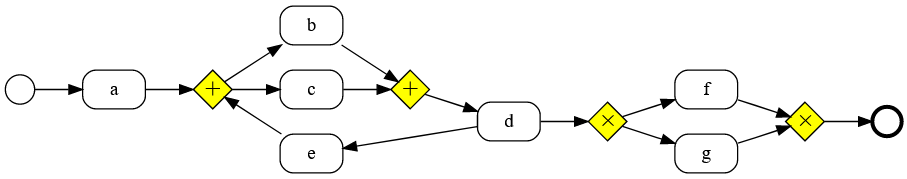
\includegraphics{Grammar-lop-example.png}}
	\caption{\label{fig:subcaption_example}Przykład problemu}
\end{figure}

Jest to możliwe za pomocą notacji: 
\{a\}and(xor(\{b\}\{c\})\{d\})\{e\}lop(\{f\}and(xor(\{b\}\{c\})\{d\})\{e\})xor(\{g\}\{h\})

Użycie powyższej notacji rodzi jednak kilka problemów, Musimy mieć produkcje 
\{a\}lo1(\{f\}and(xor(\{b\}\{c\})\{d\})\{e\})xor(\{g\}\{h\})
\clearpage

\section{Projekt systemu}

\begin{figure}[h]
	\centering{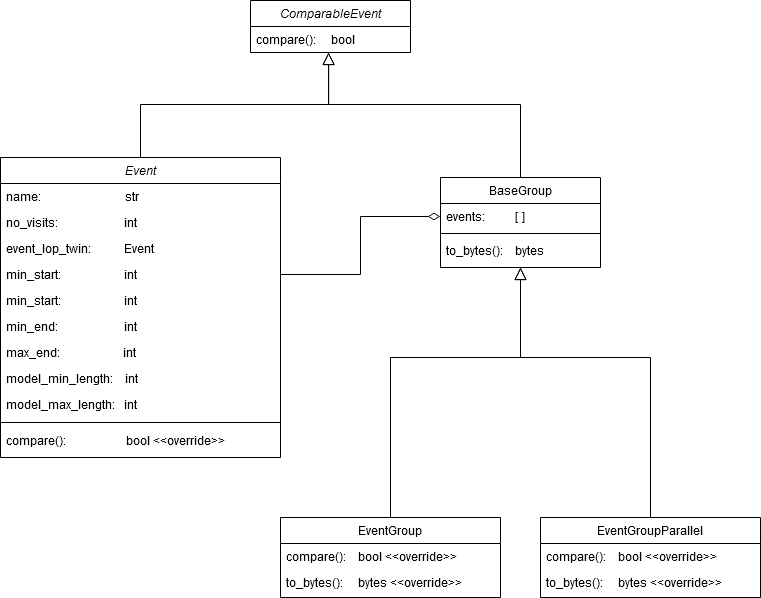
\includegraphics[scale=0.5]{EventUML.png}}
	\caption{\label{fig:subcaption_example}Event UML}
\end{figure}

Gate costam

\begin{figure}[h]
	\centering{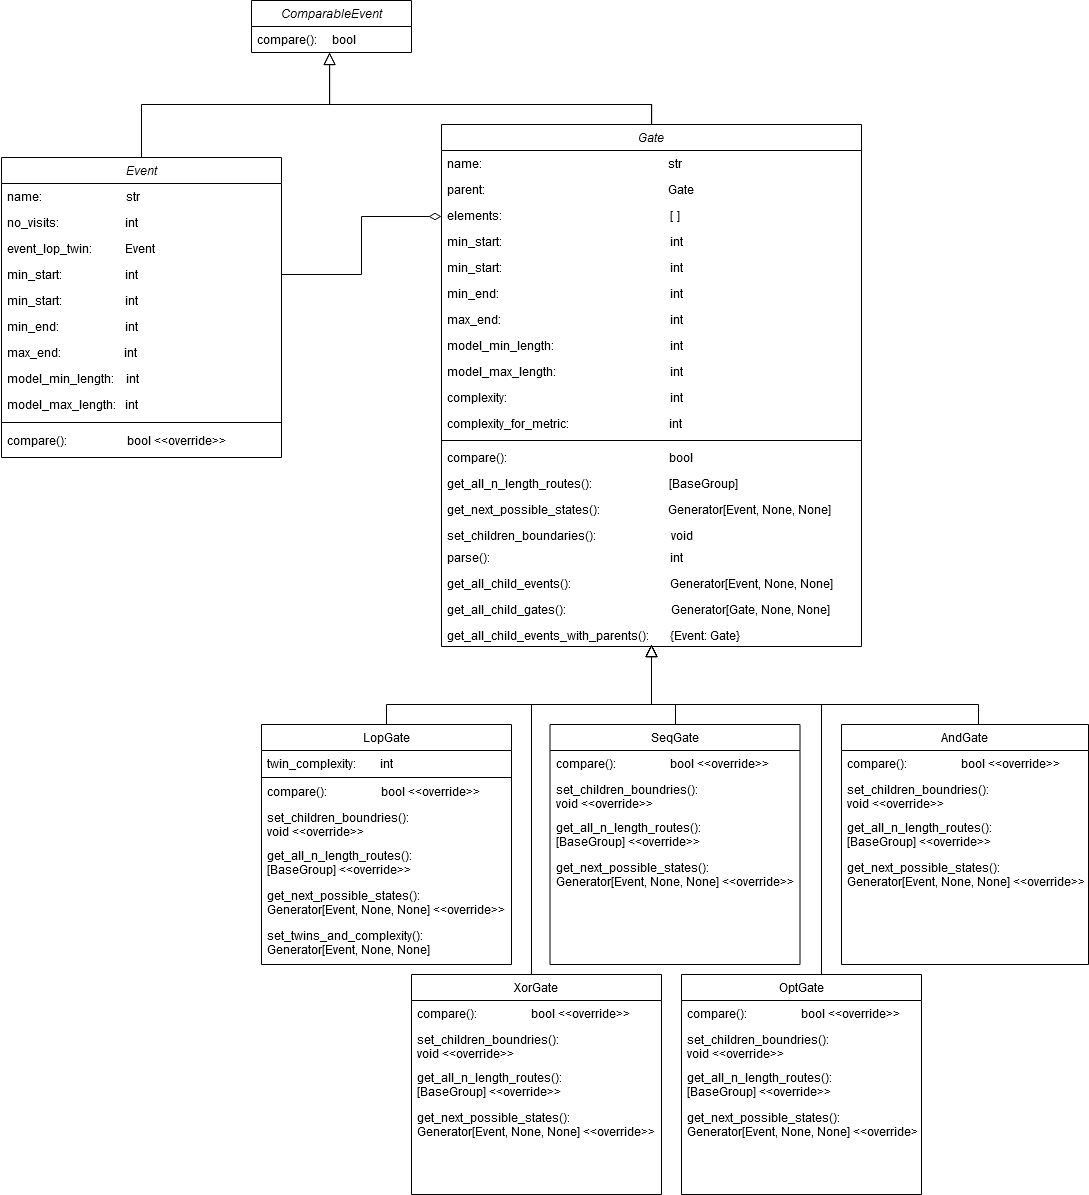
\includegraphics[scale=0.5]{GateUML.png}}
	\caption{\label{fig:subcaption_example}Gate UML}
\end{figure}

\section{Implementacja}

\subsubsection{Ogólny schemat blokowy}
\clearpage

\begin{figure}[!ht]
	\centering{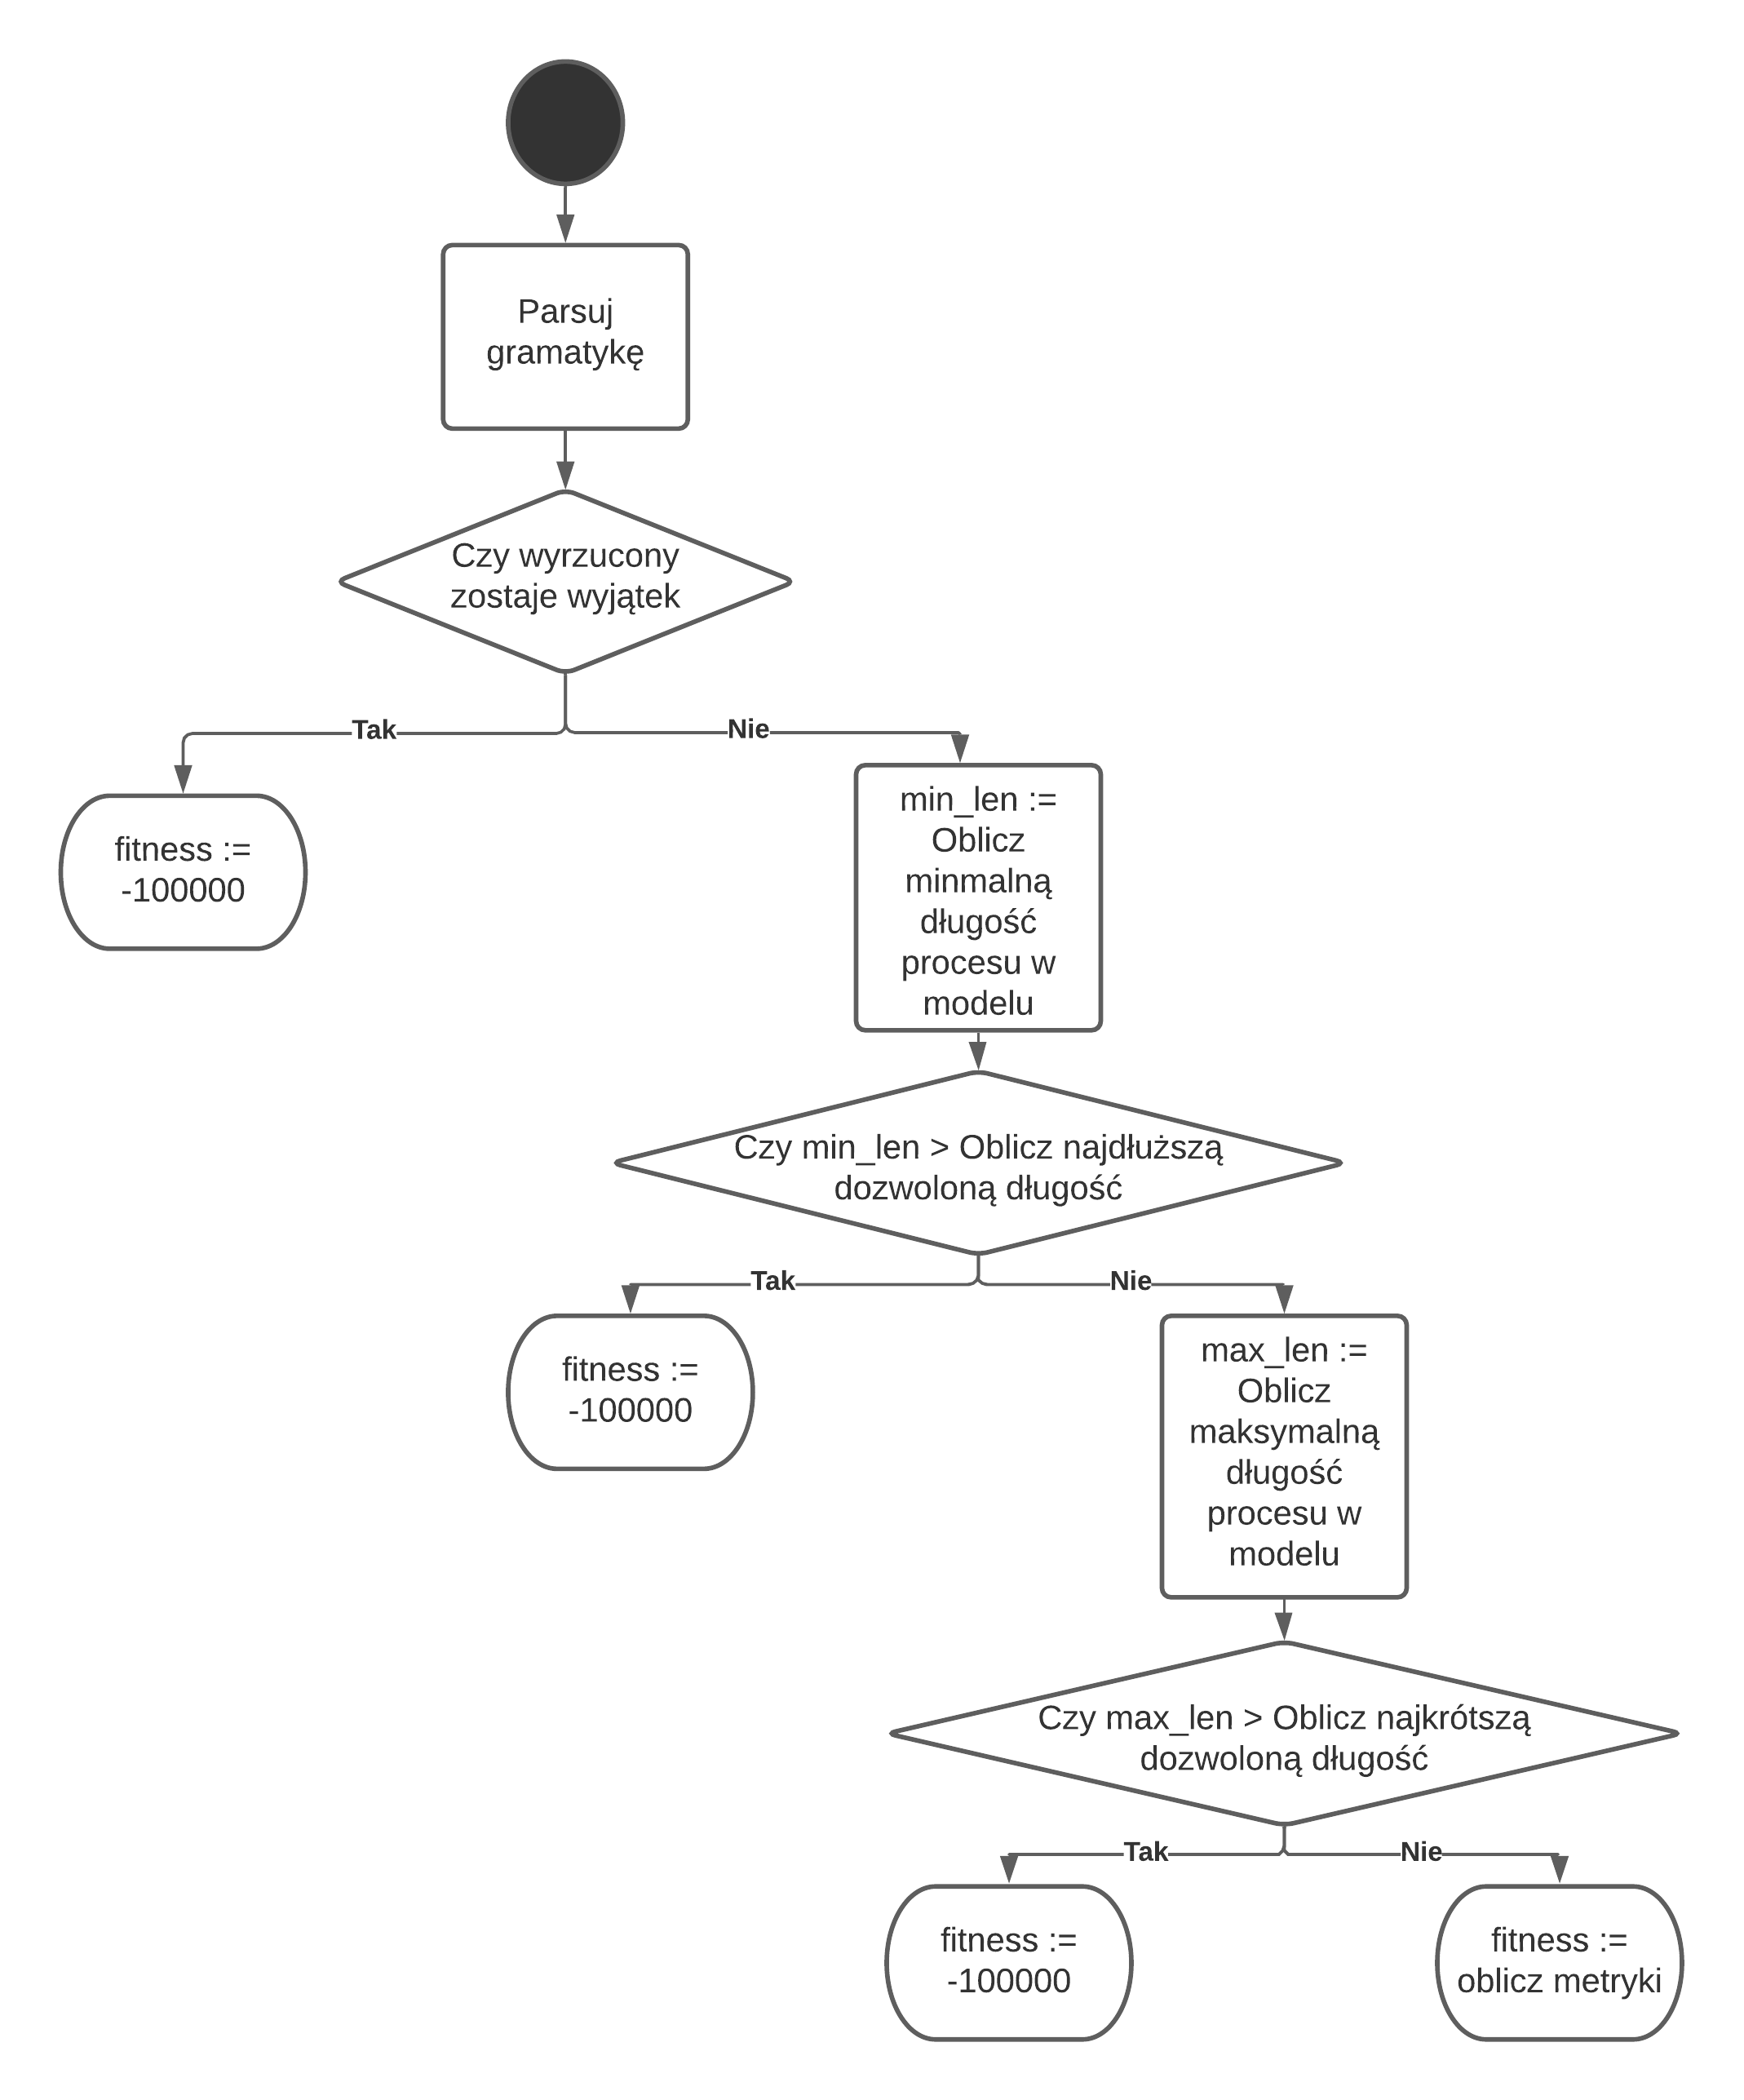
\includegraphics{Overall-flow-chart.png}}
	\caption{\label{fig:flow_chart}Ogólny schemat blokowy}
\end{figure}

\subsubsection{Parsowanie gramatyki}
Parser pozwala na przetworzenie wyników uzyskanych na drodze ewolucji gramatycznej na postać, na której łatwiej będzie operować. Rezultaty uzyskane na drodze rewolucji gramatycznej w PonyGE2 są w formie tekstowej, z którą praca byłaby niewygodna, dlatego używamy parsera, żeby otrzymać wynik w postaci drzewa obiektów Gate, którego liśćmi będą obiekty Event.
Parsując korzystamy z faktu, że przy projektowaniu gramatyki wszystkie bramki logiczne zostały oznaczone 3 literowymi symbolami, a wszystkie zdarzenia otoczone nawiasami klamrowymi. Tworząc każdy obiekt Event dodajemy informację o liczbie dzieci tego obiektu, co przyda nam się przy obliczaniu metryki precyzja.

\begin{figure}[!ht]
\lstset{caption=Parser gramatyki, captionpos=b}
\lstset{label=src:passive, frame=single}
\begin{lstlisting}
    def parsuj(wyrażenie: str) -> int:

        for i w zakresie długość_wyrażenia:
            if wyrażenia[i] == "{":
                zdarzenie := Event(wyrażenia[i + 1])
                dodaj zdarzenie do aktualnie parsowanej bramki 
                i += 2
            elif wyrażenia[i] == ")":
                return i+1
            elif i+4 < długość_wyrażenia:
                bramka := stwórz nową bramkę Gate  typu zgodnego z wyrażeniem 
                i += 3
                przeparsowane_znaki = bramka.parsuj(wyrażenie[i+4:])
                dodaj zdarzenie do aktualnie parsowanej bramki 
                i += ilość_przeparsowanych_znaków
            else:
                wyrzuć wyjątek
\end{lstlisting}
\end{figure}

\subsubsection{Obliczanie metryk}

\begin{figure}[!ht]
\lstset{caption=Obliczanie metryk, captionpos=b}
\lstset{label=src:best_result, frame=single}
\begin{lstlisting}
def oblicz_metryki(log, długość_logu, średnia_długość_procesu_w_logu, model, 
				   najkrótsza_dozwolona_długość, 
				   najdłuższa_dozwolona_długość) -> int:
    n = zaokrąglij(średnia_długość_process_w_logu)
    i = 1
    najlepszy_wynik = 0
    while n znajduje się pomiędzy największą i najmienjszą 
    	  dopuszczalną długością logu:
        if najkrótsza_dozwolona_długość <= n <= najdłuższa_dozwolona_długość:
            procesy_o_dlugosci_n = model.wyszukaj_procesy_o_określonej_długości(n)
            wszystkie_procesy = model.wyszukaj_wszystkie_procesy
            wszyscy_rodzice_procesów = model.wyszukaj_wszystkich_rodziców_procesów
            if istnieją procesy_o_dlugosci_n:
                najlepszy_błąd_lokalny = 0
                for elem w log:
                    minimalny_błąd_lokalny = 1023
                    for proces w procesy_o_dlugosci_n:
                        błąd_lokalny, ścieżka = oblicz_dopasowanie(event_group, elem)
                        if błąd_lokalny < minimalny_błąd_lokalny:
                            minimalny_błąd_lokalny = błąd_lokalny
                            najlpesza_ścieżka = ścieżka
                    najlepszy_błąd_lokalny += minimalny_błąd_lokalny
               oblicz metryki odwzorowanie, precyzja, generalizacja, prostota 
               najlepszy_wynik_lokalny = suma_obliczonych_metryk / liczba_metryk
               if najlepszy_wynik_lokalny > najlepszy_wynik:
                   najlepszy_wynik = najlepszy_wynik_lokalny
        if i % 2 == 1:
            n -= i
        else:
            n += i
        i += 1
    return najlepszy_wynik
\end{lstlisting}
\end{figure}

\subsubsection{Wyszukiwanie w modelu procesów o określonej długości}

Algorytm rekurencyjny. Implementacja rózni się w zależności od przeszukiwanej branki logicznej.
\begin{figure}[!ht]
\lstset{caption=Wyszukiwanie procesów o długości n, captionpos=b}
\lstset{label=src:get_n_length, frame=single}
\begin{lstlisting}
\end{lstlisting}
\end{figure}

\subsubsection{Obliczanie dopasowania}
Pomysł zaczerpnięty z algorytmu Needlessmann-Wunsch \cite{ea252fd3937a4a309a5e07e61e5531a7}, który jest uogólnieniem odległości Levenshteina. Rozwinięty o możliwość przeszukiwania modelu rekurencyjnie oraz o możliwość podawania listy równlogłych zdarzeń.
\begin{figure}[!ht]
\lstset{caption=Obliczanie dopasowania, captionpos=b}
\lstset{label=src:alignment_calculation, frame=single}
\begin{lstlisting}
def oblicz_dopasowanie(model, log):
    kara = {'DOPASOWANIE': 0, 'BRAK_DOPASOWANIA': -2, 'PRZERWA': -1}
    wyniki_lokalne = [None] * dlugosc_macierzy_rozwiazan
    macierz_rozwiazan = Zainicjalizuj macierz zerami
    for i in range(m):
        macierz_rozwiazan[i][0] = kara['PRZERWA'] * i
    for j in range(n):
        macierz_rozwiazan[0][j] = kara['PRZERWA'] * j
    #Wypelnij osie macierzy wlasciwymi wartosciami

    for i in range(1, m):
        if should_go_recurrent(model[i-1]):
            al_mat[i], model_results_local[i] = 
            recurrent_alignment(al_mat[i - 1], model[i - 1],
                                [x for x in substrings_of_string_reversed(log)], i)
        elif len(model[i-1]) > 1:
            al_mat[i], model_results_local[i] = 
            parallel_alignment(al_mat[i - 1], model[i - 1],
                              [x for x in substrings_of_string_reversed(log)], kara, i)
        else:
            al_mat[i][0] = al_mat[i-1][0] + penalty['GAP']
            basic_alignment(al_mat, model[i - 1], log, kara, i, n)

    model_results = get_all_tracebacks(al_mat, penalty['GAP'], model, 
    log, model_results_local)

    return macierz_rozwiazan[m-1] #ostatnia linijka, model_results
\end{lstlisting}
\end{figure}

\subsubsection{Znajdowanie ścieżki w modelu}
Potrzebne do obliczenia precyzji oraz generazlizacji.
\begin{figure}[!ht]
\lstset{caption=Znajdowanie ścieżki w modelu, captionpos=b}
\lstset{label=src:traceback, frame=single}
\begin{lstlisting}
def znajdz_sciezke(macierz_rozwiazan, model, log, rozwiazania_podmodeli):
    sciezka = []

    while i != 0:
        event_group_full_length = len(model[i - 1])
        if model_results_local[i] is not None:
            matched_flag = False
            if array[i][j] == array[i - 1][j] + event_group_full_length * penalty_gap:
                [model_result.append(None) for _ in range(event_group_full_length)]
                array[i][j] = 0
                i -= 1

            else:
                for k in range(j):
                    processes = get_not_none(model_results_local[i][k]
                    [len(model_results_local[i][k]) - (j-k)], log)
                    if array[i][j] == array[i - 1][k] + 
                    	(event_group_full_length + (j-k) - 2 * len(processes)) * penalty_gap:
                        [model_result.append(x) for x in processes]
                        for x in processes:
                            log = log.replace(x.name, "", 1)
                        [model_result.append(None) 
                         for _ in range(event_group_full_length - len(processes))]
                        array[i][j] = 0
                        i -= 1
                        j = k
                        matched_flag = True
                        break

                if not matched_flag:
                    if array[i][j] == array[i][j - 1] + penalty_gap:
                        array[i][j] = 0
                        j -= 1

        else:
            if array[i][j] == array[i - 1][j] + penalty_gap:
                model_result.append(None)
                array[i][j] = 0
                i -= 1
            elif array[i][j] == array[i][j - 1] + penalty_gap:
                array[i][j] = 0
                j -= 1
            elif array[i][j] == array[i - 1][j - 1]:
                model_result.append(model[i-1])
                log = log.replace(model[i-1].name, "", 1)
                array[i][j] = 0
                i -= 1
                j -= 1
    return sciezka
\end{lstlisting}
\end{figure}

\subsubsection{Cache}
\section{Wybór parametrów algorytmu}
